


The parallelism of Nek5000 is accomplished via domain decomposition methods and a suitable gather-scatter code. All this is implemented in such way that the user does not have to be concerned with the parallelism and only focus on the actual solvers while keepin in mind a few simple rules and routines that switch from local to global and back.
\begin{itemize}
\item Locally, the SEM is structured.

\item Globally, the SEM is unstructured.

\item Vectorization and serial performance derive from the structured aspects of the computation.

\item Parallelism and geometric flexibility derive from the unstructured, element-by-element, operator evaluation.

\item Elements, or groups of elements are distributed across processors, but an element is never subdivided.
\end{itemize}

For the most part, the global element numbering is not relevant since Nek5000 assigns it randomly but following certain rules. 

There are two types of array sizes, starting with {\color{red}l}x1, {\color{red}l}elv, etc. which give an upper bound of the arrays. And {\color{red}n}x1, {\color{red}n}elv, etc. which give the actual number of elements/grid points per processors. For the example in Fig.~\ref{fig:procsplit} we have 
\begin{itemize}
\item on proc 0, {\tt nelt=2}  (nelt = no elements in temperature domain)
\item on proc 1, {\tt nelt=3}  (nelv = no elements in fluid domain, usually = nelt)
\end{itemize}

\begin{figure}
\centering
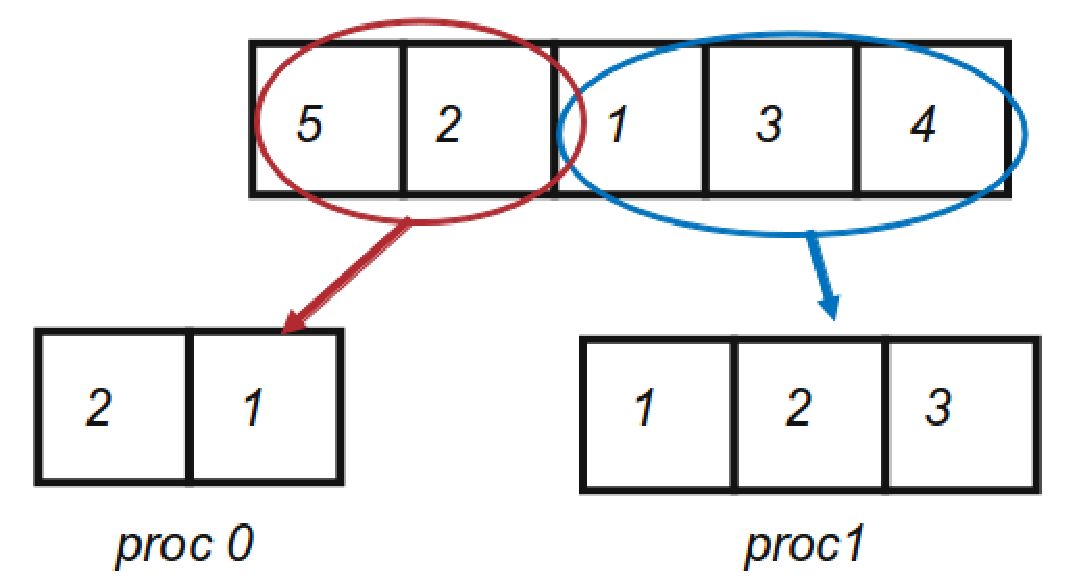
\includegraphics[scale=0.5]{serial_parallel}
\caption{A simple SEM row of elements and a potential splitting}
\label{fig:procsplit}
\end{figure}
Arrays {\tt lglel} that distinguish which processor has which elements, 

\begin{itemize}
\item on proc 0, {\tt nelt=2, lglel=(2,5)}, local element {\tt 1->2} and {\tt 2->5}
\item on proc 1, {\tt nelt=3, lglel=(1,3,4)}, local element {\tt 1->1}, {\tt 2->3} and {\tt 4->3}
\end{itemize}
		  
Now for global to local we have two common arrays (scaling as {\tt nelgt}, but only two such arrays)

\begin{itemize}
\item {\tt gllel=(1,1,2,3,2)}, assigns a global element to its local correspondent, i.e. global element {\tt 1->1}, {\tt 2->1} and {\tt 3->2} etc.
\item {\tt gllnid=(1,0,1,1,0)}, assigns a global element to its processor, i.e. {\tt 1->1}, {\tt 2->0} and {\tt 3->1} etc.
\end{itemize}



All data contiguously packed (and quad-aligned) {\tt real  u(lx1,ly1,lz1,lelt)} indicates that {\tt u} is a collection of elements, {\tt e=1,\(\ldots\),Nelt =< lelt}, each of size \((N+1)d, d=2 or 3\).

\textbf{Example: Summation}

Serial version
{\tt
s = 0 \\
do e=1,nelv \\
do iz=1,nz1 \\
do iy=1,ny1 \\
do ix=1,nx1 \\
s=s+u(ix,iy,iz,e) \\
enddo,\(\ldots\),enddo}

Second approach, serial version (works in parallel in Nek)
{\tt
n=nx1*ny1*nz1*nelv \\
s=0 \\
do i=1,n \\
s=s+u(i,1,1,1) \\
enddo
}

Nek Parallel Version

{\tt s=glsum(s,n)}

If you want a local max {\tt s=vlmax(u,n)}, or a global max {\tt s=glmax(u,n)}.


